\newpage
\section{Conocimiento previo}


\begin{section-theorem.tcb}{Ley de los Senos}{law-of-sines}
    Sea el triángulo $ABC$ con circunradio $R$.
    Entonces
    \[
        \frac{a}{\sen(\angle A)} = \frac{b}{\sen(\angle B)} = \frac{c}{\sen(\angle C)} = 2R.
    \]
\end{section-theorem.tcb}

\textbf{Pista:} Considerar las antípodas de los vértices en el circuncírculo de $\triangle ABC$, notar ciertas igualdades de ángulos por cuadriláteros cíclicos y luego utilizar la definción del seno para el triángulo rectángulo.


\begin{section-theorem.tcb}{Teorema de bisectriz generalizada}{ratio-lemma}
    Dado el triángulo $ABC$, sea el punto $X$ en $BC$.
    Entonces se cumple que
    \[
        \frac{BX}{XC} = \frac{AB}{AC} \cdot \frac{\sen(\angle BAX)}{\sen(\angle XAC)}.
    \]
\end{section-theorem.tcb}

\textbf{Pista:} Utilizar el~\refTheorem{\ref{t:law-of-sines}} y la siguiente identidad trigonométrica:
\[
    \text{Si}\ \alpha + \beta = 180^\circ\text{,}\ \text{entonces}\ \sen(\alpha) = \sen(\beta).
\]

\begin{section-property}[Potencia de un punto exterior]\label{power-external-point}
Sean $AD$ y $CD$ dos rectas que se intersecan en $X$ tales que $X - A - B$ y $X - C - D$.
Entonces el cuadrilátero $ABCD$ es cíclico si y solo si
\[
    \overline{XA} \cdot \overline{XB} = \overline{XC} \cdot \overline{XD}.
\]
\end{section-property}

\begin{multicols}{2}
    \begin{proof}
        Rápidamente nos damos cuenta de que $\angle CXB = \angle AXD\quad (\ast).$

        Entonces $ABCD$ es cíclico
        \begin{align*}
            &\iff \angle ABC = \angle ADC\\
            &\iff \angle XBC = \angle ADX\\
            &\overset{(\ast)}{\iff} \triangle XBC \sim \triangle XDA \ \overset{(\ast)}{\iff} \ \frac{\overline{XB}}{\overline{XC}} = \frac{\overline{XD}}{\overline{XA}}\\[2mm]
            &\iff \overline{XA} \cdot \overline{XB} = \overline{XC} \cdot \overline{XD}. \qedhere
        \end{align*}
    \end{proof}
    \begin{figure}[H]
        \centering
        \definecolor{ttttff}{rgb}{0.2,0.2,1}
%dash pattern=on 5pt off 2pt
%[fill = white, rounded corners = 4pt, inner sep = 1pt]
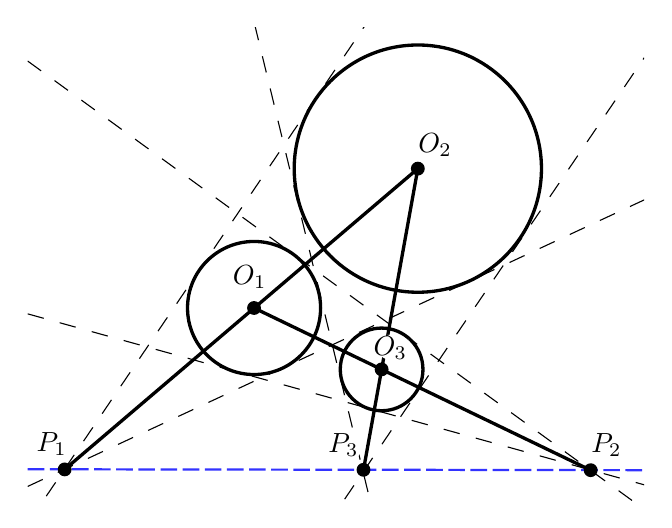
\begin{tikzpicture}[scale = 0.5]
    \clip(4.47,-5.82) rectangle (20.13,6.18);
    \draw [line width=1.2pt] (10.22,-0.94) circle (1.69cm);
    \draw [line width=1.2pt] (13.46,-2.5) circle (1.05cm);
    \draw [line width=1.2pt] (14.38,2.6) circle (3.14cm);
    \draw [line width=1.2pt] (5.41,-5.04)-- (14.38,2.6);
    \draw [line width=1.2pt] (14.38,2.6)-- (13,-5.05);
    \draw [line width=1.2pt] (10.22,-0.94)-- (18.77,-5.06);
    \draw [color = ttttff, dash pattern=on 6pt off 2pt, line width=0.8pt, domain=4.47:20.13] plot(\x,{(-67.19-0.02*\x)/13.36});
    \draw [dash pattern=on 6pt off 6pt,domain=4.47:20.13] plot(\x,{(-41.75--2.57*\x)/5.53});
    \draw [dash pattern=on 6pt off 6pt,domain=4.47:20.13] plot(\x,{(-44.52--5.05*\x)/3.42});
    \draw [dash pattern=on 6pt off 6pt,domain=4.47:20.13] plot(\x,{(-32.25--1.96*\x)/1.33});
    \draw [dash pattern=on 6pt off 6pt,domain=4.47:20.13] plot(\x,{(-27.15--2.31*\x)/-0.56});
    \draw [dash pattern=on 6pt off 6pt,domain=4.47:20.13] plot(\x,{(-40.25--3.41*\x)/-4.69});
    \draw [dash pattern=on 6pt off 6pt,domain=4.47:20.13] plot(\x,{(-0.84--1.55*\x)/-5.59});
    \begin{scriptsize}
        \normalsize
        \fill [color=black] (10.22,-0.94) circle (5pt);
        \draw[color=black] (10.11,-0.15) node[fill = white, rounded corners = 4pt, inner sep = 1pt] {$O_1$};
        \fill [color=black] (14.38,2.6) circle (5pt);
        \draw[color=black] (14.82,3.2) node {$O_2$};
        \fill [color=black] (13.46,-2.5) circle (5pt);
        \draw[color=black] (13.68,-1.95) node[fill = white, rounded corners = 8pt, inner sep = 0.5pt] {$O_3$};
        \fill [color=black] (5.41,-5.04) circle (5pt);
        \draw[color=black] (5.08,-4.4) node {$P_1$};
        \fill [color=black] (18.77,-5.06) circle (5pt);
        \draw[color=black] (19.17,-4.43) node {$P_2$};
        \fill [color=black] (13,-5.05) circle (5pt);
        \draw[color=black] (12.49,-4.43) node[fill = white, rounded corners = 4pt, inner sep = 1pt] {$P_3$};
    \end{scriptsize}
\end{tikzpicture}
    \end{figure}
\end{multicols}